\documentclass[11pt]{article}
\usepackage{amsmath}
\usepackage{amssymb}
\usepackage{graphicx}
\usepackage{tabularx}
\usepackage{fancyhdr}
\usepackage{lastpage}

% Page layout
\usepackage[top=1in, bottom=1in, left=1in, right=1in]{geometry}

% Header and footer
\pagestyle{fancy}
\fancyhf{}
\rfoot{Page \thepage}
\renewcommand{\headrulewidth}{0pt}

% Modified Question command with left-aligned number
\newcommand{\questiona}[2]{
    \noindent\textbf{Q#2.} #1 \hfill \textbf{[1 Mark]}
}

\newcommand{\questionb}[2]{
    \noindent\textbf{Q#2.} #1 \hfill \textbf{[2 Marks]}
}

\begin{document}

% Title section with horizontal line
\begin{center}
    \Large\textbf{GATE 2018 - Chemical Engineering (CH)} \\
    \large\textbf{General Aptitude and Technical Questions} \\
    \rule{\textwidth}{0.5pt} % Horizontal line below heading
\end{center}

\vspace{0.5cm}

% General Aptitude Section
\section*{General Aptitude}

\questiona{"When she fell down the \_\_\_\_\_, she received many \_\_\_\_\_ but little help." The words that best fill the blanks in the above sentence are}{1}
\begin{enumerate}
    \item[(A)] stairs, stares  
    \item[(B)] stairs, stairs  
    \item[(C)] stares, stairs  
    \item[(D)] stares, stares  
\end{enumerate}

\questiona{"In spite of being warned repeatedly, he failed to correct his \_\_\_\_\_ behaviour." The word that best fills the blank in the above sentence is}{2}
\begin{enumerate}
    \item[(A)] rational  
    \item[(B)] reasonable  
    \item[(C)] errant  
    \item[(D)] good  
\end{enumerate}

\questiona{For \(0 \leq x \leq 2\pi\), \(\sin x\) and \(\cos x\) are both decreasing functions in the interval \_\_\_\_\_.}{3}
\begin{enumerate}
    \item[(A)] \(\left(0, \frac{\pi}{2}\right)\)  
    \item[(B)] \(\left(\frac{\pi}{2}, \pi\right)\)  
    \item[(C)] \(\left(\pi, \frac{3\pi}{2}\right)\)  
    \item[(D)] \(\left(\frac{3\pi}{2}, 2\pi\right)\)  
\end{enumerate}

\questiona{The area of an equilateral triangle is \(\sqrt{3}\). What is the perimeter of the triangle?}{4}
\begin{enumerate}
    \item[(A)] 2  
    \item[(B)] 4  
    \item[(C)] 6  
    \item[(D)] 8  
\end{enumerate}

\questiona{Arrange the following three-dimensional objects in the descending order of their volumes: (i) A cuboid with dimensions 10 cm, 8 cm and 6 cm (ii) A cube of side 8 cm (iii) A cylinder with base radius 7 cm and height 7 cm (iv) A sphere of radius 7 cm}{5}
\begin{enumerate}
    \item[(A)] (i), (ii), (iii), (iv)  
    \item[(B)] (ii), (i), (iv), (iii)  
    \item[(C)] (iii), (ii), (i), (iv)  
    \item[(D)] (iv), (iii), (ii), (i)  
\end{enumerate}

\questionb{An automobile travels from city A to city B and returns to city A by the same route. The speed of the vehicle during the onward and return journeys were constant at 60 km/h and 90 km/h, respectively. What is the average speed in km/h for the entire journey?}{6}
\begin{enumerate}
    \item[(A)] 72  
    \item[(B)] 73  
    \item[(C)] 74  
    \item[(D)] 75  
\end{enumerate}

\questionb{A set of 4 parallel lines intersect with another set of 5 parallel lines. How many parallelograms are formed?}{7}
\begin{enumerate}
    \item[(A)] 20  
    \item[(B)] 48  
    \item[(C)] 60  
    \item[(D)] 72  
\end{enumerate}

\questionb{To pass a test, a candidate needs to answer at least 2 out of 3 questions correctly. A total of 6,30,000 candidates appeared for the test. Question A was correctly answered by 3,30,000 candidates. Question B was answered correctly by 2,50,000 candidates. Question C was answered correctly by 2,60,000 candidates. Both questions A and B were answered correctly by 1,00,000 candidates. Both questions B and C were answered correctly by 90,000 candidates. Both questions A and C were answered correctly by 80,000 candidates. If the number of students answering all questions correctly is the same as the number answering none, how many candidates failed to clear the test?}{8}
\begin{enumerate}
    \item[(A)] 30,000  
    \item[(B)] 2,70,000  
    \item[(C)] 3,90,000  
    \item[(D)] 4,20,000  
\end{enumerate}

\questionb{If \(x^2 + x - 1 = 0\) what is the value of \(x^4 + \frac{1}{x^4}\)?}{9}
\begin{enumerate}
    \item[(A)] 1  
    \item[(B)] 5  
    \item[(C)] 7  
    \item[(D)] 9  
\end{enumerate}

\questionb{In a detailed study of annual crow births in India, it was found that there was relatively no growth during the period 2002 to 2004 and a sudden spike from 2004 to 2005. In another unrelated study, it was found that the revenue from cracker sales in India which remained fairly flat from 2002 to 2004, saw a sudden spike in 2005 before declining again in 2006. The solid line in the graph below refers to annual sale of crackers and the dashed line refers to the annual crow births in India. Choose the most appropriate inference from the above data.}{10}
\begin{center}
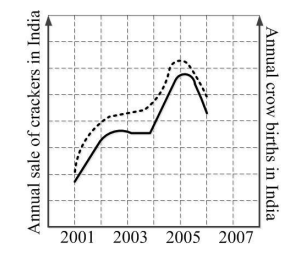
\includegraphics[width=0.5\textwidth]{figures/Q10.png}
\end{center}
\begin{enumerate}
    \item[(A)] There is a strong correlation between crow birth and cracker sales.  
    \item[(B)] Cracker usage increases crow birth rate.  
    \item[(C)] If cracker sale declines, crow birth will decline.  
    \item[(D)] Increased birth rate of crows will cause an increase in the sale of crackers.  
\end{enumerate}

% Technical Section
\section*{Technical Section}

\questiona{Consider the following two equations:
\[\frac{dx}{dt} + x + y = 0\]
\[\frac{dy}{dt} - x = 0\]
The above set of equations is represented by}{1}
\begin{enumerate}
    \item[(A)] \(\frac{d^2 y}{dt^2} - \frac{dy}{dt} - y = 0\)  
    \item[(B)] \(\frac{d^2 x}{dt^2} - \frac{dx}{dt} - y = 0\)  
    \item[(C)] \(\frac{d^2 y}{dt^2} + \frac{dy}{dt} + y = 0\)  
    \item[(D)] \(\frac{d^2 x}{dt^2} + \frac{dx}{dt} + y = 0\)  
\end{enumerate}

\questiona{The fourth order Runge-Kutta (RK4) method to solve an ordinary differential equation \(\frac{dy}{dx} = f(x, y)\) is given as
\[y(x + h) = y(x) + \frac{1}{6}(k_1 + 2k_2 + 2k_3 + k_4)\]
For a special case when the function \(f\) depends solely on \(x\), the above RK4 method reduces to}{2}
\begin{enumerate}
    \item[(A)] Euler's explicit method  
    \item[(B)] Trapezoidal rule  
    \item[(C)] Euler's implicit method  
    \item[(D)] Simpson's 1/3 rule  
\end{enumerate}

\questiona{A watch uses two electronic circuits (ECs). Each EC has a failure probability of 0.1 in one year of operation. Both ECs are required for functioning of the watch. The probability of the watch functioning for one year without failure is}{3}
\begin{enumerate}
    \item[(A)] 0.99  
    \item[(B)] 0.90  
    \item[(C)] 0.81  
    \item[(D)] 0.80  
\end{enumerate}

\questiona{The figure which represents \(y = \frac{\sin x}{x}\) for \(x > 0\) (\(x\) in radians) is}{4}
\begin{center}
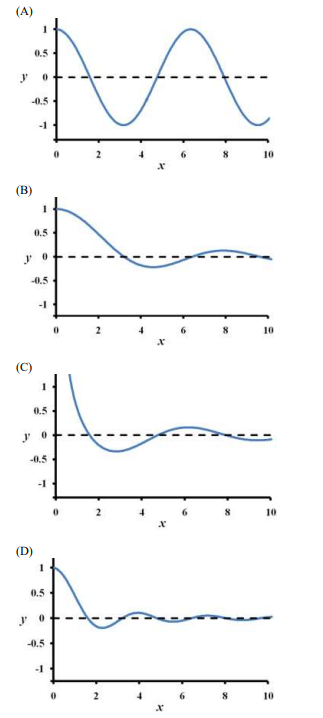
\includegraphics[width=0.5\textwidth]{figures/Q4.png}
\end{center}

\questiona{The terminal velocity of a spherical particle in gravitational settling under Stokes' regime varies}{5}
\begin{enumerate}
    \item[(A)] linearly with the particle diameter  
    \item[(B)] linearly with the viscosity of the liquid  
    \item[(C)] directly with the square of particle diameter  
    \item[(D)] inversely with the density of particle  
\end{enumerate}

\questiona{Critical speed of a ball mill depends on}{6}
\begin{enumerate}
    \item[(A)] the radius of the mill (shell) and the radius of the particles  
    \item[(B)] the radius of the mill (shell) and the density of the particles  
    \item[(C)] the radius of the balls and the radius of the particles  
    \item[(D)] the radius of the balls and the radius of the mill (shell)  
\end{enumerate}

\questiona{Economy of evaporators used for concentrating sugarcane juice is}{7}
\begin{enumerate}
    \item[(A)] kg of concentrated juice produced per kg of steam supplied  
    \item[(B)] kg of steam supplied per kg of sugarcane juice fed  
    \item[(C)] kg of water vaporized per kg of steam supplied  
    \item[(D)] kg of sugarcane juice fed per kg of water vaporized  
\end{enumerate}

\questiona{Segmental baffles in a 2-4 shell and tube heat exchanger}{8}
\begin{enumerate}
    \item[(A)] change the flow pattern of the tube side fluid and increase the overall heat transfer coefficient  
    \item[(B)] increase the heat transfer coefficient in the shell side and support the tubes  
    \item[(C)] help to reduce the thermal expansion of the tubes and increase the heat transfer coefficient in the tube side  
    \item[(D)] increase the number of passes in the shell side and increase the heat transfer coefficient in the tube side  
\end{enumerate}

\questiona{In connection with petroleum refining, identify the incorrect statement among the following options.}{9}
\begin{enumerate}
    \item[(A)] Desalting of crude oil is done before processing it in atmospheric distillation unit  
    \item[(B)] A stream of hydrogen is produced in catalytic reforming of naphtha  
    \item[(C)] Asphalt used for paving is a petroleum product  
    \item[(D)] Cetane number indicates the quality of petrol / motor spirit  
\end{enumerate}

\questiona{Polyvinyl chloride is produced by}{10}
\begin{enumerate}
    \item[(A)] co-polymerization  
    \item[(B)] addition-type kinetics  
    \item[(C)] reacting chlorine with polyethylene  
    \item[(D)] reacting hydrochloric acid with polyethylene  
\end{enumerate}

\questiona{The molecular formula of the predominant chemical compound in commercial sugar is}{11}
\begin{enumerate}
    \item[(A)] $C_{12}H_{22}O_{11}$  
    \item[(B)] $C_{12}H_{24}O_{12} $ 
    \item[(C)] $C_6H_{10}O_5 $ 
    \item[(D)] $C_6H_{12}O_6  $
\end{enumerate}

\questiona{Two packed towers are designed for the same mass velocity of the gas. The first has liquid and gas flow rates of 30 kg/s and 1.2 kg/s, respectively, while the corresponding flow rates in the second tower are 67.5 kg/s and 1.8 kg/s. The ratio of the design diameter of the wider tower to that of the narrower tower is}{12}
\begin{enumerate}
    \item[(A)] 2  
    \item[(B)] 1.8  
    \item[(C)] 1.5  
    \item[(D)] 1.225  
\end{enumerate}

\questiona{The Annual Fixed Charges (AFC) and Annual Utilities Costs (AUC) of a distillation column being designed are expressed in terms of the reflux ratio (R) as
\[ \text{AFC (Rs. Lakh)} = 641 \times R^2 - 1796 \times R + 1287 + 1/(R - 1.16) \]
\[ \text{AUC (Rs. Lakh)} = 80 + 62.5 \times R \]
The reflux ratio \( R_{\text{opt}} \) for optimizing the total cost of the distillation column may be found by solving}{13}
\begin{enumerate}
    \item[(A)] \( 1282 \times R_{\text{opt}} - 1796 - 1/(R_{\text{opt}} - 1.16)^2 = 0 \)  
    \item[(B)] \( 62.5 + 1282 \times R_{\text{opt}} - 1796 - 1/(R_{\text{opt}} - 1.16)^2 = 0 \)  
    \item[(C)] \( 80 + 62.5 \times R_{\text{opt}} + 641 \times R_{\text{opt}}^2 - 1796 \times R_{\text{opt}} + 1287 + 1/(R_{\text{opt}} - 1.16) = 0 \)  
    \item[(D)] \( 80 + 62.5 \times R_{\text{opt}} - 641 \times R_{\text{opt}}^2 + 1796 \times R_{\text{opt}} - 1287 - 1/(R_{\text{opt}} - 1.16) = 0 \)  
\end{enumerate}

\questiona{Consider the following properties: (P) temperature (Q) specific gravity (R) chemical potential (S) volume. The option which lists ALL the intensive properties is}{14}
\begin{enumerate}
    \item[(A)] P  
    \item[(B)] P and Q  
    \item[(C)] P, Q and R  
    \item[(D)] P, Q, R and S  
\end{enumerate}

\questiona{Liquid phase isomerization of o-xylene to p-xylene using a zeolite catalyst was carried out in a CSTR. Three sets of kinetic data at different temperatures and stirring speeds were obtained as shown below.
\begin{center}
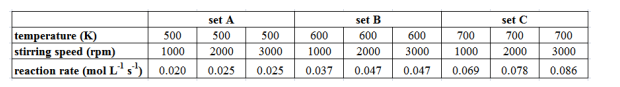
\includegraphics[width=1\textwidth]{figures/Q15.png}
\end{center}
The operating condition at which the reaction rate is not controlled by external mass transfer resistance is}{15}
\begin{enumerate}
    \item[(A)] T = 500 K; rpm = 3000  
    \item[(B)] T = 600 K; rpm = 1000  
    \item[(C)] T = 700 K; rpm = 1000  
    \item[(D)] T = 700 K; rpm = 2000  
\end{enumerate}

\questiona{Choose the correct statement. In viscose rayon manufacturing process,}{16}
\begin{enumerate}
    \item[(A)] carbon disulphide used as reactant for xanthate formation is regenerated in a later step  
    \item[(B)] caustic soda used as reactant for steeping of cellulose is regenerated in a later step  
    \item[(C)] sulphuric acid is used in steeping process of cellulose  
    \item[(D)] the spun viscose rayon is hardened in an alkali bath  
\end{enumerate}

\questiona{The reactant (M) is converted into product (N) in the presence of catalyst in a fixed bed reactor. All the flow rates (F, G, H, P and R) in mol/s, and mole fraction of reactant (M) in these streams $(x_F, x_G, x_H, x_P and x_R)$ are shown in the diagram.
\begin{center}
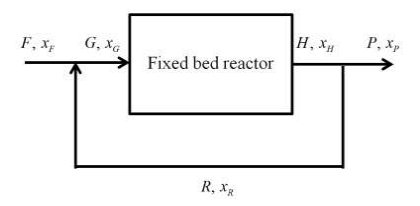
\includegraphics[width=0.5\textwidth]{figures/Q17.png}
\end{center}
The overall fractional conversion is}{17}
\begin{enumerate}
    \item[(A)] \(\frac{x_G G - x_H H}{x_G G}\)  
    \item[(B)] \(\frac{x_G G - x_P P}{x_G G}\)  
    \item[(C)] \(\frac{x_F F - x_H H}{x_F F}\)  
    \item[(D)] \(\frac{x_F F - x_P P}{x_F F}\)  
\end{enumerate}

\questiona{A first-order process having a transfer function, \(G_p = \frac{2}{7s + 1}\) is controlled by a proportional controller with gain of 3.2. The process time constant is in minutes. Addition of the integral control action with an integral time constant of 5 minutes leads to increase in}{18}
\begin{enumerate}
    \item[(A)] offset  
    \item[(B)] speed of response  
    \item[(C)] order of the closed loop system  
    \item[(D)] proportional band  
\end{enumerate}

\questiona{According to the surface renewal theory, the unit of fractional rate of surface renewal is}{19}
\begin{enumerate}
    \item[(A)] m\(^2\) s\(^{-2}\)  
    \item[(B)] m\(^2\) s\(^{-1}\)  
    \item[(C)] m s\(^{-1}\)  
    \item[(D)] s\(^{-1}\)  
\end{enumerate}

\questiona{For absorption of H\(_2\)S from a mixture with hydrocarbon vapour into an aqueous alkanolamine solution, the liquid phase mass transfer resistance is}{20}
\begin{enumerate}
    \item[(A)] significantly higher than that of the gas phase  
    \item[(B)] negligible compared to that of the gas phase  
    \item[(C)] equal to that of the gas phase  
    \item[(D)] dependent on the gas phase mass transfer resistance  
\end{enumerate}

\questiona{For a chemical reaction, the ratio of rate constant at 500 K to that at 400 K is 2.5. Given R = 8.314 J mol\(^{-1}\) K\(^{-1}\), the value of activation energy (in kJ/mol) is}{21}
\begin{enumerate}
    \item[(A)] 10.5  
    \item[(B)] 12.0  
    \item[(C)] 15.2  
    \item[(D)] 18.4  
\end{enumerate}

\questiona{Pitot tube is used to measure}{22}
\begin{enumerate}
    \item[(A)] liquid level in a tank  
    \item[(B)] flow velocity at a point  
    \item[(C)] angular deformation  
    \item[(D)] vorticity  
\end{enumerate}

\questiona{A venturi meter is installed to measure the flow rate of water in a 178 mm diameter (ID) pipe. The throat diameter is 102 mm. The differential pressure measured using a manometer is 154.3 kN/m\(^2\). The data given are: discharge coefficient = 0.98; water density = 1000 kg/m\(^3\). The volumetric flow rate of water (in m\(^3\)/s) is \_\_\_\_\_.}{23}

\questiona{The ammonia (NH\(_3\)) oxidation process occurs over a catalyst as
\[ 4 NH_3 + 5O_2 \rightarrow 6H_2O + 4NO \]
Air is supplied such that oxygen (O\(_2\)) is 20\% in excess of that required for complete conversion of NH\(_3\). The mole fraction of O\(_2\) in inlet gas mixture (NH\(_3\) + air) is \_\_\_\_\_ (rounded off to third decimal place)}{24}

\questiona{The initial water level in a tank is 4 m. When the valve located at the bottom is opened, the rate of change of water level (L) with respect to time (t) is, \(\frac{dL}{dt} = -k\sqrt{t}\), where \(k = 0.6 \, \text{m s}^{-3/2}\). The level of water (in m) in the tank at time 0.5 s after opening the valve is \_\_\_\_\_ (rounded off to second decimal place).}{25}

\questionb{Match the equipment in Column A with the corresponding process in Column B}{26}
\begin{center}
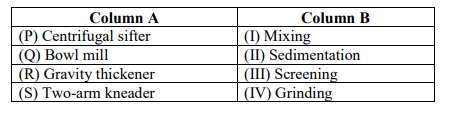
\includegraphics[width=0.5\textwidth]{figures/Q26.png}
\end{center}
\begin{enumerate}
    \item[(A)] P-I, Q-IV, R-II, S-III  
    \item[(B)] P-III, Q-IV, R-II, S-I  
    \item[(C)] P-IV, Q-I, R-II, S-III  
    \item[(D)] P-IV, Q-III, R-I, S-II  
\end{enumerate}

\questionb{In the year 2005, the cost of a shell and tube heat exchanger with 68 m\(^2\) heat transfer area was Rs. 12.6 Lakh. Chemical Engineering Index for cost in 2005 was 509.4 and now the index is 575.4. Based on index of 0.6 for capacity scaling, the present cost (in Lakhs of rupees) of a similar heat exchanger having 100 m\(^2\) heat transfer area is estimated to be}{27}
\begin{enumerate}
    \item[(A)] 17.94  
    \item[(B)] 19.94  
    \item[(C)] 20.94  
    \item[(D)] 22.94  
\end{enumerate}

\questionb{A furnace installed at a cost of Rs. 24 Lakh is expected to serve its useful life of 5 years. Salvage value of the furnace is Rs. 8 Lakh. The interest rate compounded annually is 8\%. The estimated capitalized cost (in Lakhs of rupees) is}{28}
\begin{enumerate}
    \item[(A)] 30  
    \item[(B)] 34.09  
    \item[(C)] 34.9  
    \item[(D)] 58.09  
\end{enumerate}

\questionb{G denotes the Gibbs free energy of a binary mixture, nT denotes the total number of moles present in the system, \(\mu_i\) is the chemical potential of the ith component (\(\mu_1 \neq \mu_2\) and \(\mu_2 > 0\)) and xi is the mole fraction of the ith component. The correct variation of G/nT (in J/mol) at constant temperature and pressure is given by}{29}
\begin{center}
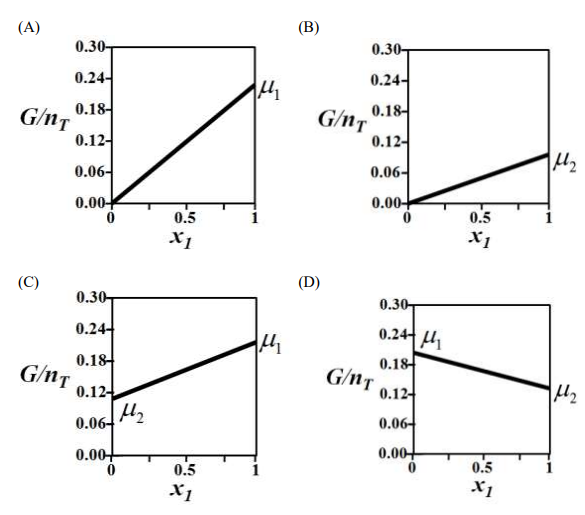
\includegraphics[width=0.8\textwidth]{figures/Q29.png}
\end{center}

\questionb{A person is drowning in sea at location R and the lifeguard is standing at location P. The beach boundary is straight and horizontal, as shown in the figure.
\begin{center}
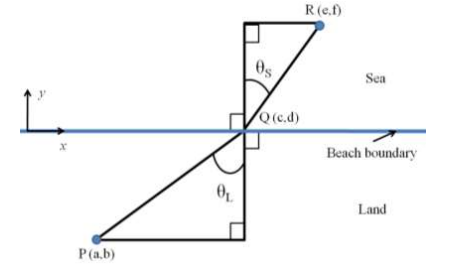
\includegraphics[width=0.5\textwidth]{figures/Q30.png}
\end{center}
The lifeguard runs at a speed of \(V_L\) and swims at a speed of \(V_S\). In order to reach to the drowning person in optimum time, the lifeguard should choose point Q such that}{30}

\begin{enumerate}
    \item[(A)] \(\frac{\sin^2 \theta_L}{\sin^2 \theta_S} = \frac{V_S}{V_L}\)  
    \item[(B)] \(\frac{\sin \theta_L}{\sin \theta_S} = \frac{V_S}{V_L}\)  
    \item[(C)] \(\frac{\sin^2 \theta_L}{\sin^2 \theta_S} = \frac{V_L}{V_S}\)  
    \item[(D)] \(\frac{\sin \theta_L}{\sin \theta_S} = \frac{V_L}{V_S}\)  
\end{enumerate}

\questionb{The decay ratio for a system having complex conjugate poles as \(\left( -\frac{1}{10} + j \frac{2}{15} \right)\) and \(\left( -\frac{1}{10} - j \frac{2}{15} \right)\) is}{31}
\begin{enumerate}
    \item[(A)] 7×10\(^{-1}\)  
    \item[(B)] 8×10\(^{-2}\)  
    \item[(C)] 9×10\(^{-3}\)  
    \item[(D)] 10×10\(^{-4}\)  
\end{enumerate}

\questionb{Match the items in Column A with the items in Column B}{32}
\begin{center}
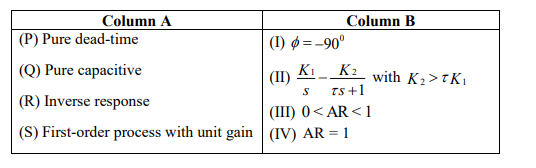
\includegraphics[width=0.5\textwidth]{figures/Q32.png}
\end{center}
\begin{enumerate}
    \item[(A)] P-II, Q-III, R-IV, S-I  
    \item[(B)] P-III, Q-II, R-IV, S-I  
    \item[(C)] P-I, Q-IV, R-II, S-III  
    \item[(D)] P-IV, Q-I, R-II, S-III  
\end{enumerate}

\questionb{In a laboratory batch setup, reaction of P over a catalyst was studied at various temperatures. The reactions occurring are \(P \rightarrow 2Q\) and \(P \rightarrow R\). At the end of one hour of operation, the batch contains \(x_P\), \(x_Q\) and \(x_R\) mole fractions of P, Q and R components, respectively. The mole fractions of product components (\(x_Q\) and \(x_R\)) were found to vary linearly with temperature as given in the figure.
\begin{center}
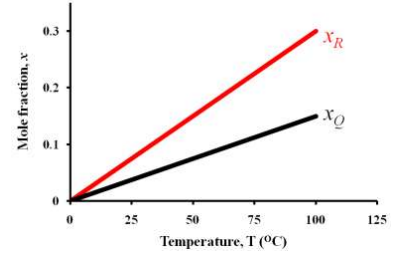
\includegraphics[width=0.5\textwidth]{figures/Q33.png}
\end{center}
If the yield of Q based on reactant P consumed (\(Y_Q\)) at 25 °C was found to be 0.40, then the value of \(Y_Q\) at 60 °C is \_\_\_\_\_ (rounded off to second decimal place).}{33}
\vspace{0.5cm}

\questionb{An insulated storage tank contains 1000 kg liquid of specific heat 10 kJ kg\(^{-1}\) K\(^{-1}\). The liquid is heated by saturated steam, condensing in a helical coil at a temperature of 180 °C. The heat transfer area of the coil is 0.1 m\(^2\). If the overall heat transfer coefficient is constant at 1000 W m\(^{-2}\) K\(^{-1}\), then the time (in hours) required to raise the temperature of the liquid in the tank from 20 °C to 80 °C is \_\_\_\_\_ (rounded off to second decimal place).}{34}
\vspace{0.5cm}

\questionb{The wall of a pipe of radius 1 m is at a uniform temperature of 200 °C, and is covered by insulation of thickness 0.1 m. The ambient air outside the insulated pipe is at 20 °C and has heat transfer coefficient of 10 W m\(^{-2}\) K\(^{-1}\). The thermal conductivity of the insulation material is 0.05 W m\(^{-1}\) K\(^{-1}\). If the heat transfer occurs at steady state, the temperature (in °C) of the outer surface of insulation is \_\_\_\_\_ (rounded off to second decimal place).}{35}
\vspace{0.5cm}


\questionb{Vapour bubbles are formed in the nucleate boiling regime at a frequency of 10 bubbles per second per nucleation site. There are 100 nucleation sites per m\(^2\) of heating area. The latent heat of vapourization and the density of vapour under the operating condition are 1000 kJ/kg and 1 kg/m\(^3\) respectively. The diameter of each bubble is 10\(^{-3}\) m. Assume that the entire heat supplied is used for vapour generation. The heat flux (in Watt per m\(^2\) of heating area) is \_\_\_\_\_ (rounded off to third decimal place).}{36}
\vspace{0.5cm}


\questionb{Under isothermal condition, a vertical tube of length L = 100 m contains a gas of molecular weight equal to 60. The pressure and temperature at the top of the tube are 100 kPa and 25 °C respectively. Consider the universal gas constant and acceleration due to gravity as 8.314 J mol\(^{-1}\) K\(^{-1}\) and 9.81 m s\(^{-2}\) respectively. If the gas is ideal, the pressure (in kPa) at the bottom of the tube will be \_\_\_\_\_ (rounded off to third decimal place).}{37}
\vspace{0.5cm}

\questionb{At a shear rate of 10 s\(^{-1}\), the apparent viscosity of a non-Newtonian liquid was found to be 1 Pa s. At a shear rate of 100 s\(^{-1}\), the apparent viscosity of the same liquid was found to be 0.5 Pa s. If the liquid follows power law behavior, the apparent viscosity (in Pa s) at a shear stress of 10 N m\(^{-2}\) is \_\_\_\_\_ (rounded off to two decimal place).}{38}
\vspace{0.5cm}

\questionb{A CSTR and a PFR of equal volume are connected in series as shown below to carry out a first-order, isothermal, liquid phase reaction 
\begin{center}
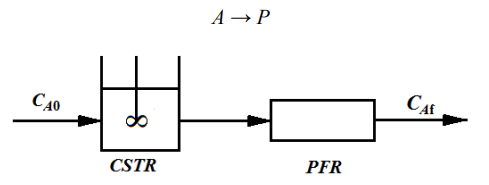
\includegraphics[width=0.5\textwidth]{figures/Q39.png}
\end{center}
The rate constant is 0.2 s\(^{-1}\). The space-time is 5 s for both the reactors. The overall fractional conversion of A is \_\_\_\_\_ (rounded off to third decimal place).}{39}
\vspace{0.5cm}

\questionb{The elementary second-order liquid phase reaction A + B → C + D is carried out in an isothermal plug flow reactor of 2 m\(^3\) volume. The inlet volumetric flow rate is 10 m\(^3\)/h. The initial concentrations of both A and B are 2 kmol/m\(^3\). The rate constant is given as 2.5 m\(^3\) kmol\(^{-1}\) h\(^{-1}\). The percentage conversion of A is \_\_\_\_\_.}{40}
\vspace{0.5cm}
\questionb{It is decided to extract A from a feed containing 20 mol\% A and 80 mol\% B in two ideal cross-current stages as shown below, using equal amount of pure solvent C in each stage. 
\begin{center}
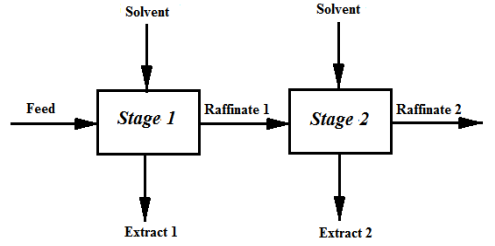
\includegraphics[width=0.5\textwidth]{figures/Q41.png}
\end{center}
Components B and C are immiscible. 60\% of A in the feed is extracted in Stage 1. The equilibrium relation is given by Y* = 1.5 X where, X = moles of A per mole of B in raffinate, Y* = moles of A per mole of C in extract in equilibrium with raffinate. The mol \% of A in raffinate from Stage 2 is \_\_\_\_\_ (rounded off to second decimal place).}{41}
\vspace{0.5 cm}

\questionb{A binary distillation column is designed by McCabe-Thiele method to get a distillate mole fraction of 0.9. The enriching section operating line has an intercept with y-axis at 0.3 mole fraction. The ratio of liquid to vapour molar flow rate in the enriching section is \_\_\_\_\_ (rounded off to third decimal place).}{42}
\vspace{0.5 cm}

\questionb{A fiberboard sheet (1.5 m × 2.0 m × 15 mm) is being dried by suspending it horizontally in a current of hot, dry air. The edges are insulated so that drying takes place only from the top and bottom surfaces. The wet sheet weighing 16 kg with initial moisture content of 60\% loses moisture at a constant rate of \(1.25 \times 10^{-5}\) kg m\(^{-2}\) s\(^{-1}\) until the moisture content falls to 30\%. All moisture contents are on dry basis. The time required for drying during constant rate period (in hour) is \_\_\_\_\_ (rounded off to third decimal place).}{43}
\vspace{0.5 cm}

\questionb{Consider the following transfer function:
\[G(s) = \frac{3}{(5s+1)^2}\]
where, the natural period of oscillation is in min. The amplitude ratio at a frequency of 0.5 rad/min is \_\_\_\_\_ (rounded off to second decimal place).}{44}
\vspace{0.5 cm}

\questionb{For a closed-loop system, consider the following transfer functions: process \(G_p(s)\), controller \(G_c(s)\), measuring device \(G_m(s)\), and final control element \(G_f(s)\):
\[G_p(s) = \frac{2}{7s+1}; G_c(s) = 2; G_m(s) = 1; G_f(s) = 1\]
The offset in the closed loop response due to a unit step change introduced in the set point of the output variable is \_\_\_\_\_.}{45}
\vspace{0.5 cm}

\questionb{If \(y = e^{-x^2}\) then the value of \(\lim_{x \to +\infty} \frac{1}{x} \frac{dy}{dx}\) is \_\_\_\_\_.}{46}
\vspace{0.5 cm}

\questionb{For the matrix \(A = \begin{pmatrix} \cos \theta & -\sin \theta \\ \sin \theta & \cos \theta \end{pmatrix}\) if det stands for the determinant and \(A^T\) is the transpose of A then the value of det (\(A^T A\)) is \_\_\_\_\_.}{47}
\vspace{0.5 cm}

\questionb{An azeotropic mixture of ethanol and water is to be separated in a distillation column using benzene as an entrainer. At the column operating conditions, two liquid phases are formed on a tray. The degree(s) of freedom of the system for the choice of intensive properties at equilibrium is(are) \_\_\_\_\_.}{48}
\vspace{0.5 cm}

\questionb{The volume of liquid filled in a spherical storage tank of radius R is computed from height of liquid, h, in the outside tube (neglecting the volume of liquid in the outside tube) as
\[V = \frac{\pi h^2 (3R - h)}{3}\]

\begin{center}
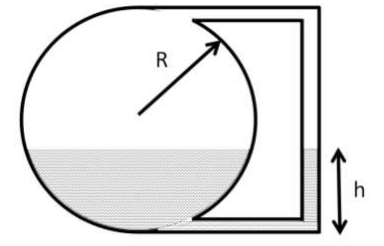
\includegraphics[width=0.5\textwidth]{figures/Q49.png}
\end{center}
The estimate of liquid height (in m) to store V = 30 m\(^3\) of water in R = 3 m tank, after performing ONE iteration of Secant method, using 1 m and 3 m as two initial guesses of liquid height is \_\_\_\_\_ (rounded off to second decimal place).}{49}
\vspace{0.5cm}
\questionb{In a closed piston-cylinder system, methane was observed to obey the following equation of state
\[P (V - nb) = nRT\]
where b = 0.029 m\(^3\)/mol. The temperature and volume are 500 °C and 5 m\(^3\) respectively for 100 moles of methane. At this state of the system, the isobaric rate of change of temperature with volume (in °C/m\(^3\)) is \_\_\_\_\_ (rounded off to second decimal place).}{50}
\vspace{0.5cm}

\questionb{A set of standard stainless steel pipes, each of internal diameter 26.65 mm and 6000 mm length, is used to make a plug flow reactor by joining them in series to carry out degradation of polyethylene. Seven such pipes are required to obtain a conversion of 66\% at 450 K. The minimum number of standard 8000 mm long pipes of the same internal diameter to be procured for obtaining at least 66\% conversion under the same reaction conditions is \_\_\_\_\_.}{51}
\vspace{0.5cm}

\questionb{Hydrogenation of benzene is to be carried out using Ni (density = 8910 kg/m\(^3\)) as catalyst, cast in the form of non-porous hollow cylinders. The reaction occurs on all the surfaces of the hollow cylinder. During an experiment, one such cylinder is suspended in the reactant stream. If the observed rate of reaction is 0.39 mol (m\(^2\) of catalyst surface)\(^{-1}\) min\(^{-1}\), then the rate of reaction in mol (kg of catalyst)\(^{-1}\) min\(^{-1}\) is \_\_\_\_\_ (rounded off to three decimal places).}{52}
\begin{center}
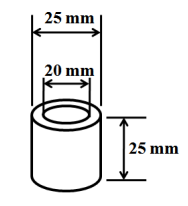
\includegraphics[width=0.5\textwidth]{figures/Q52.png}
\end{center}

\vspace{0.5cm}
\questionb{ The humidity of air at a dry-bulb temperature of 65 °C is 0.025 kg water/kg dry air. The latent heat of vaporization of water at 0 °C is 2500 kJ/kg. The psychrometric ratio of air is 0.95 kJ (kg dry air)\(^{-1}\) K\(^{-1}\). Considering 0 °C as reference temperature, the enthalpy of air (in kJ/kg) at its adiabatic saturation temperature of 35 °C is \_\_\_\_\_\_ (rounded off to two decimal places).}{53}

\vspace{0.5cm}

\questionb{ In a roll crusher, rolls of diameter 1 m each are set in such a manner that minimum clearance between the crushing surfaces is 15 mm. If the angle of nip is 31°, the maximum diameter of the particle (in mm) which can be crushed is \_\_\_\_\_\_ (rounded off to third decimal place).}{54}

\vspace{0.5cm}

\questionb {A hot liquid is to be cooled in a 1-1 shell and tube heat exchanger from 80 °C to 50 °C. Cooling water enters the tube side at 30 °C, and exits at 45 °C. The properties of the liquids are constant. Also, the overall heat transfer coefficient is same for counter-current and co-current modes. The percentage saving in heat transfer area for counter-current option with respect to the area of co-current option is \_\_\_\_\_\_ (rounded off to third decimal place).}{55}

\vspace{5cm}
\begin{center}
\textbf{END OF THE QUESTION PAPER}
\rule{\textwidth}{0.5pt} 
\end{center}

\end{document}